\documentclass[12pt]{article}
\usepackage{amsfonts}
\usepackage{fancyhdr}
\usepackage[a4paper, top=2.5cm, bottom=2.5cm, left=2.2cm, right=2.2cm]{geometry}
\usepackage{times}
\usepackage{amsmath}
\usepackage{changepage}
\usepackage{amssymb}
\usepackage{graphicx}%
\setcounter{MaxMatrixCols}{30}
\newtheorem{theorem}{Theorem}
\newtheorem{acknowledgement}[theorem]{Acknowledgement}
\newtheorem{algorithm}[theorem]{Algorithm}
\newtheorem{axiom}{Axiom}
\newtheorem{case}[theorem]{Case}
\newtheorem{claim}[theorem]{Claim}
\newtheorem{conclusion}[theorem]{Conclusion}
\newtheorem{condition}[theorem]{Condition}
\newtheorem{conjecture}[theorem]{Conjecture}
\newtheorem{corollary}[theorem]{Corollary}
\newtheorem{criterion}[theorem]{Criterion}
\newtheorem{definition}[theorem]{Definition}
\newtheorem{example}[theorem]{Example}
\newtheorem{exercise}[theorem]{Exercise}
\newtheorem{lemma}[theorem]{Lemma}
\newtheorem{notation}[theorem]{Notation}
\newtheorem{problem}[theorem]{Problem}
\newtheorem{proposition}[theorem]{Proposition}
\newtheorem{remark}[theorem]{Remark}
\newtheorem{solution}[theorem]{Solution}
\newtheorem{summary}[theorem]{Summary}
\usepackage{enumitem}
\usepackage[utf8]{inputenc}
\newenvironment{proof}[1][Proof]{\textbf{#1.} }{\ \rule{0.5em}{0.5em}}
\usepackage{tikz}
\usepackage{graphicx}
\usepackage{wrapfig}
\usepackage{float}
\usepackage{datetime}
\newdateformat{specialdate}{\twodigit{\THEDAY}.\twodigit{\THEMONTH}.\THEYEAR}
\usepackage{amssymb}
\usepackage{ifsym}
\usepackage{listings}
\usepackage{lipsum}  

\newcommand{\Q}{\mathbb{Q}}
\newcommand{\R}{\mathbb{R}}
\newcommand{\C}{\mathbb{C}}
\newcommand{\Z}{\mathbb{Z}}

\begin{document}
	
	\title{1. Übung}
	\author{Timo Bergerbusch 344408, Andreas Nikulin 332065}
	\date{\specialdate\today}
	\maketitle
	
	
	\section{Exercise 1.1}
			
	
		 \begin{enumerate}
			\item Layers:\\
			\begin{minipage}{.6\textwidth}
					\textbf{Logical data structures}:\\
					concepts: translate and optimize queries\\
					interface: set-oriented interface: relations, tuples, views \\
					
					\textbf{Logical access structures}:\\
					concepts: manage cursor, sort components and dictionary\\
					interface: record oriented interface: records, sets, keys, access paths\\
					
					\textbf{Storage Structures}:\\
					concepts: manage record and index\\
					interface: internal record interface: records, B* trees\\
					
					\textbf{Page assignment}:\\
					concepts: manage buffer and segments\\
					interface: system buffer interface: pages, segments\\
					
					\textbf{Memory assignment structures}:\\
					concepts: manage files and external memory\\
					interface: file interface: blocks, files\\
					
					\textbf{physical volume}:\\
					interface: device interface: tracks, cylinders, channels\\
			\end{minipage}
			\begin{minipage}{.3\textwidth}
				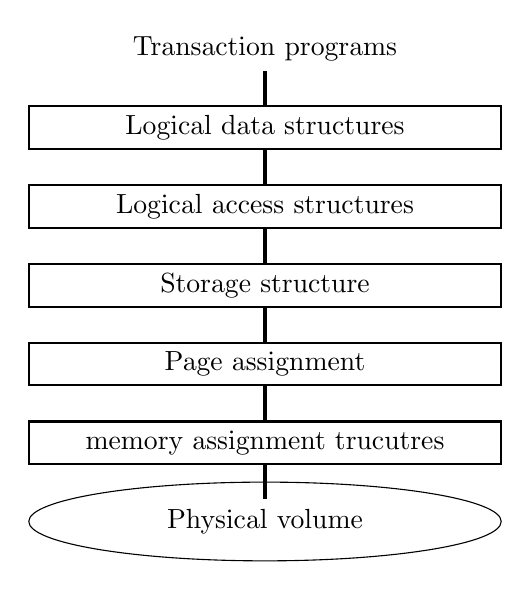
\begin{tikzpicture}
				\node (0) {Transaction programs};
				\node[draw, rectangle, thick, minimum width=6cm, minimum height=.5cm, below of =0] (1) {Logical data structures};
				\node[draw, rectangle, thick, minimum width=6cm, minimum height=.5cm,below of=1] (2) {Logical access structures};
				\node[draw, rectangle, thick, minimum width=6cm, minimum height=.5cm,below of=2] (3) {Storage structure};
				\node[draw, rectangle, thick, minimum width=6cm, minimum height=.5cm,below of=3] (4) {Page assignment};
				\node[draw, rectangle, thick, minimum width=6cm, minimum height=.5cm,below of=4] (5) {memory assignment trucutres};
				\draw (0,-6) ellipse (3cm and .5cm) node (6) {Physical volume};
				
				\draw[draw=black, ultra thick] (0) edge (1);
				\draw[draw=black, ultra thick] (1) edge (2);
				\draw[draw=black, ultra thick] (2) edge (3);
				\draw[draw=black, ultra thick] (3) edge (4);
				\draw[draw=black, ultra thick] (4) edge (5);
				\draw[draw=black, ultra thick] (5) edge (6);
				\end{tikzpicture}
			\end{minipage}
		
			\item Order: $e \rightarrow b \rightarrow d \rightarrow a \rightarrow c$
			
			\item \begin{enumerate}[label=(\alph*)]
				\item \textbf{data independence}: the view on the data is independent of its organized structure inside of the DB\\
					  \textbf{Physical data independence}: the underlying logical organization is independent of the physical representation. So restructuring or changing the implemented structure does not affect the schema\\
					  \textbf{logical data independence}: the logical schema might change without any affect on the external schema
				\item Data independence is important because it can provide an encapsulated split between development of programs on an external given structure independent of its internal handling.  
				\item answer:
					\begin{figure}[H]
						\centering
						\includegraphics[scale=0.6]{Exercise113c.PNG}
					\end{figure}
					
			\end{enumerate}
		\end{enumerate}
	\section{Exercise 1.2}
	
	\begin{enumerate}
		\item relational algebra
			\begin{enumerate}[label=(\alph*)]
				\item $\pi_{code}(\sigma_{percentage=100\land Continent='Africa'}(encompasses))$
				\item $\pi_{lakeName}( riverthrough \bowtie_{river=river1} \rho_{river1\leftarrow river}(\sigma_{Country="F"}(located)))$
				\item $\pi_{name}(sea)  - \pi_{name}(sea \bowtie_{depth1 > depth}(\rho_{name1,depth1}(sea)))$
				\item $\rho_{CountryWithTheHighestMountain}(\pi_{name}\\
							(\pi_{name}(Mountain) - \pi_{name}( Mountain \bowtie_{elevation<elevation1} \rho_{elevation1 \leftarrow elevation}(Mountain))\\
							\bowtie geo\_Mountain \bowtie Country
							)$
			\end{enumerate}
		\item SQL queries
			\lstinputlisting[
			language=SQL,
			showspaces=false,
			basicstyle=\ttfamily,
			numbers=left,
			numberstyle=\tiny,
			commentstyle=\color{gray}
			]{Exercise1.2.2.sql}
	\end{enumerate}
\end{document}


















